\begin{table} [h]
\begin{center}
\begin{tabular}{|c|c|}
	\hline
	$Номер результата измерений j$ & $Результат измерений x_j$\\
	\hline
	1 & 15.61 \\ 
	\hline
	2 & 20.71 \\ 
	\hline
	3 & 21.68 \\ 
	\hline
	4 & 22.28 \\ 
	\hline
	5 & 23.22 \\ 
	\hline
	6 & 24.14 \\ 
	\hline
	7 & 24.59 \\ 
	\hline
	8 & 26.18 \\ 
	\hline
	9 & 26.23 \\ 
	\hline
	10 & 27.59 \\ 
	\hline
	11 & 27.88 \\ 
	\hline
	12 & 28.74 \\ 
	\hline
	13 & 29.34 \\ 
	\hline
	14 & 30.86 \\ 
	\hline
	15 & 32.08 \\ 
	\hline
\end{tabular}
\end{center}
\caption{Результаты измерений, упорядоченные по значению, n = 15}
\end{table} 

\begin{figure}[h]
\center{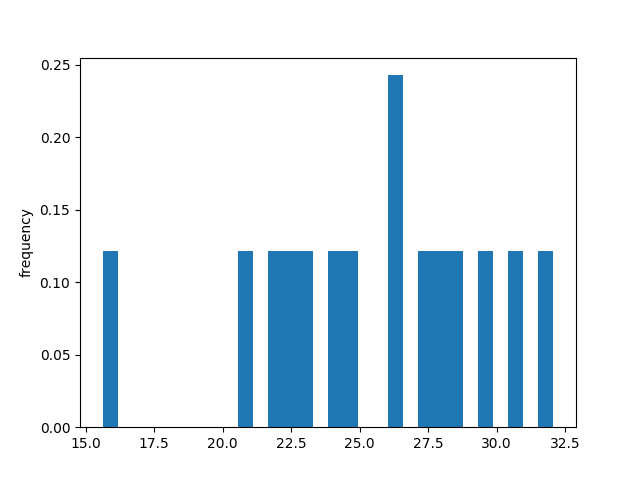
\includegraphics[width=1\linewidth]{normCramer.png}}
\caption{Пробная выборка, n = 15}
\label{fig:box20}
\end{figure}


\begin{table} [h]
\resizebox{0.7\textwidth}{!}{\begin{minipage}{\textwidth}
\begin{tabular}{|c|c|c|c|c|c|c|c|c|c|}
	\hline
	$j$ & $A_j=\frac{2j-1}{2n}$ & $B_j=F(x_j)$  & $C_j=ln(B_j)$ & $D_j=(A_j)(C_j)$ & $E_j=1-A_j$ & $F_j=1-B_j$ & $G_j=ln(F_j))$ & $H_j=(E_j)(G_j)$ & $I_j=(D_j)+(H_j)$\\
	\hline
	 1 & 0.033 &  0.011723  & -4.44618 &  -0.14820 &  0.9666 &  0.988277 & -0.01179  & -0.01139 & -0.1596\\
	 \hline
	 2 &  0.100 &  0.138600   & -1.97616 &  -0.19761 &  0.9000 &  0.861400 & -0.14919  & -0.13427 & -0.33189\\
	 \hline
	 3 &  0.167 &  0.194259   &  -1.63856 & -0.27309 &  0.8333 &  0.805741 & -0.21599  & -0.17999 & -0.45308\\
	 \hline
	 4 & 0.233  &  0.234672  &  -1.44956 &  -0.33823 &  0.7666 &  0.765328 & -0.26745  & -0.20504 & -0.54327\\
	 \hline
	 5 & 0.300 &  0.306372   &  -1.18295 &  -0.35488 &  0.7000 &  0.693628 & -0.36582  & -0.25607 & -0.61096\\
	 \hline
	 6 & 0.367  &  0.384609   &  -0.95552 &  -0.35036 &  0.6333 &  0.615391 & -0.48549  & -0.30748 & -0.65784\\
	 \hline
	 7 & 0.433  &  0.424918  & -0.85586 &  -0.37087 &  0.5666 &  0.575082 & -0.55324  & -0.31350 & -0.68437\\
	 \hline
	 8 & 0.500 &  0.570788  & -0.56073 & -0.28036 &  0.5000 &  0.429212 & -0.84580  & -0.42290 & -0.70327\\
	 \hline
	 9 & 0.567  & 0.575324   &  -0.55282 &  -0.31326 &  0.4333 &  0.424676 & -0.85642  & -0.37111 & -0.68438\\
	 \hline
	 10 & 0.633  &  0.693032  &  -0.36667 &  -0.23223 &  0.3666 &  0.306968 & -1.18101  & -0.43303 & -0.66526\\
	 \hline
	 11 &  0.700  & 0.716180   &  -0.33382 &  -0.23367 &  0.3000 &  0.283820 & -1.25941  & -0.37782 & -0.61150\\
	 \hline
	 12 & 0.767  &  0.779474   &  -0.24913 &  -0.19100 &  0.2333 &  0.220526 & -1.51174  & -0.35273 & -0.54374\\
	 \hline
	 13 & 0.833  &  0.818371   &  -0.20043 &  -0.16703 &  0.1666 &  0.181629 & -1.70579  & -0.28429 & -0.45133\\
	 \hline
	 14 & 0.900  &  0.896291   &  -0.10949 &  -0.09854 &  0.1000 &  0.103709 & -2.26616 & -0.22661 & -0.32515\\
	 \hline
	 15 & 0.967  &  0.938565  &  -0.06340 &  -0.06129 &  0.0333 &  0.061435 & -2.78977 &  -0.09299 & -0.15428\\
	\hline
	$\sum$ & & & & & & & & & -7.57998\\
	\hline
\end{tabular}
\end{minipage} }
\caption{Результаты промежуточных вычислений значения статистики $n\Omega_n^2$ по формуле \ref{eq:Г1}, n = 15} \label{tab:nomega} 
\end{table} 







